\begin{center}\large\textbf{Readings: 18.1-18.7}\\
\normalsize \end{center}
\large ~\hrulefill
~\\

\textbf{Motivating Example:}\\
Experiment investigating pesticide (3 levels) on yield of corn.  
\begin{itemize}
\item 6 plots of land used
\item CRD done (each of 3 pesticides randomly assigned to 2 plots)
\end{itemize}

\begin{center}
\begin{tabular}{ccc}
plot &    pest &     y\\\hline
1&        1 &    53.4\\
2&        1 &    46.5\\
1&        2 &    54.3\\
2 &       2 &    57.2\\
1 &       3 &    55.9\\
2  &      3 &    57.4\\
\end{tabular}
\end{center}

Analysis?  One-way ANOVA model:
$$Y_{ij}=\mu+\alpha_{i}+E_{ij}$$
\begin{itemize}
\item $\mu$ is overall mean
\item $\alpha_i$ is effect of pesticide $i$
\item $E_{ij}$ random effect of plot (iid $N(0,\sigma^2)$)
\end{itemize}
Test for pesticide is
$$F=MS(Trt)/MS(E)\mbox{  i.e.  }F=MS(Pesticide)/MS(Plot)$$~\\

\textbf{Split-plot experiment}\\
Consider the same experiment except, after you've assigned the pesticide, you break each plot into 4 `subplots.'  You randomly assign the 4 levels of a second factor, irrigation, to the subplots.\\
\begin{center}
\begin{tabular}{cccccc}
pest &   plot &    Yield at Irr 1 &    Yield at Irr 2 &     Yield at Irr 3 &     Yield at Irr 4\\\hline
1 &      1   &     53.4 &   53.8 &   58.2  &  59.5\\
1 &      2  &      46.5 &   51.1 &   49.2  &  51.3\\
2 &      1  &      54.3 &   56.3 &   60.4  &  64.5\\
2 &      2  &      57.2 &   56.9 &   61.6  &  66.8\\
3 &      1  &      55.9 &   58.6 &   62.4  &  64.5\\
3 &      2  &      57.4  &  60.2 &   57.2  &  62.7\\
\end{tabular}
\end{center}

Total number of data points?\\~\\~\\
Is usual two-way ANOVA model appropriate here?  Why or why not?\\~\\
No! Errors in two-way model are assumed independent.  Here, observations on the same plot are probably more alike than observations on separate plots. \\~\\~\\
\textbf{Completely Randomized Split Plot model}
$$Y_{ijk}=\mu+\alpha_i+S_{(i)k}+\beta_{j}+(\alpha\beta)_{ij}+E_{ijk}$$
\begin{itemize}
\item $i=1,2,3$ pesticides (generally, $i=1,...,a$)
\item $j=1,2,3,4$ irrigation (generally, $j=1,...,b$)
\item $k=1,2$ plots (generally $k=1,...,r$)
\item $S_{(i)j}\sim^{iid}N(0,\sigma^2_S)$ `whole plot error' = random effect for plot $j$ with pesticide $i$\\
Nested as plots are different for each level of pesticide.
\item $E_{ijk}\sim^{iid}N(0,\sigma^2)$ 'subplot error' = random effect between subplots  (independent of $S$)
\end{itemize}

\newpage

Definitions
\begin{itemize}
\item Experimental Unit - Unit on which a factor has its levels assigned
\item $A$ - \textbf{Whole plot factor (WPF)} (also called a {\em between plots} or {\em between subjects}  factor)
\item \textbf{Whole Plots (WP)} - E.U.'s for WPF
\item $B$ - \textbf{Subplot factor (SPF)} (also called a {\em within plots} or {\em within subjects} factor)
\item \textbf{Subplots (SP)} - E.U.'s for SPF
\end{itemize}
In terms of a repeated measures study (over time) on `subjects'.  Whole plots = `subjects', time = Subplot factor.\\~\\

Suggestion: draw a picture of the layout when possible!\\~\\~\\~\\~\\~\\~\\~\\~\\

This is a mixed effects model!  One possible way to make inference?  Look at expected mean squares!\\~\\
\begin{Beqnarray*}
Y_{ijk} &=& \underbrace{\mu + \alpha_i + \beta_j+(\alpha\beta)_{ij}}_{\mu_{ij}: (\mbox{fixed component})} + \overbrace{S_{(i)k} + E_{ijk}}^{\mbox{ random error components}}.\\
\end{Beqnarray*}

Here, $i=1,\ldots,a$ and $j=1,\ldots,b$ and $k=1,\ldots,r$ where $r$ denotes the number of plots treated with level $i$ of factor $a$.  (Note: Ott and Longnecker uses different subscripts.)\\~\\

\begin{center}
\begin{tabular}{lrc}  \hline
Source & df & EMS \\ \hline
$A$ (Pesticide) & $a-1=2$ & $\sigma^2 + b \sigma_s^2 + br \psi_A^2$ \\
Plot($A$) & $(r-1)a=(2-1)3=3$ & $\sigma^2 + b \sigma_s^2$ \\
B (Treatments) & $b-1=3$ & $\sigma^2 + ra \psi_B^2$\\ 
$A\times B$ & $(a-1)(b-1)=6$ & $\sigma^2 + r \psi_{AB}^2$\\ 
$B\times $plot(A) (Subplot error) & $(b-1)(r-1)a=9$ & $\sigma^2$\\ 
Total & $abr-1=23$\\ \hline
\end{tabular}
\end{center}

\newpage

Test for the Whole plot factor is 
$$F=MS(A)/MS(Plot(A))\mbox{    equivalent to one way ANOVA test!}$$
Test for the sub plot factor is 
$$F=MS(B)/MS(E)$$
and test for interaction is
$$F=MS(AB)/MS(E)$$~\\

The variance of an observation is 
$$Var(Y_{ijk})=\sigma^2_S+\sigma^2$$
Covariance between two observations on same plot is
$$Cov(Y_{ij_1k},Y_{ij_2k})=\sigma^2_S$$~\\

Model allows for the correlation of observations on same plot!
$$Corr(Y_{ij_1k},Y_{ij_2k})=\frac{\sigma^2_S}{\sigma^2+\sigma^2_S}$$




For the corn yields data,
\begin{center}
\begin{tabular}{crcccc}  \hline
Source & MS & df & EMS & F & $p-$value\\ \hline
$A:$ Pesticide & 128.1 & $2$ & $\sigma^2 + b \sigma_s^2 + br \psi_A^2$ & 3.9 & 0.1452\\
Whole plot error & $MS[S(A)]=32.6$ & $3$ & $\sigma^2 + b \sigma_s^2$ & 10.1 & 0.0031\\
B: treatments & 60.2 & $3$ & $\sigma^2 + ra \psi_B^2$ & $18.7$ & 0.0003\\ 
$A\times B$ & 4.1 & $6$ & $\sigma^2 + r \psi_{AB}^2$ & 1.3 & 0.3607 \\ 
$B\times $plot(A) & $MS[E]=3.2$ & $9$ & $\sigma^2$  \\
(Subplot error) & \\ \hline
Total & & $23$\\ \hline
\end{tabular}
\end{center}
\bigkn

\begin{itemize}
\item $MS[S(A)]$ denotes mean square for WHOLE plots (nested in $A$) 
\item $MS[E]$ denotes error or subplot mean square 
\end{itemize}

\newpage
Analysis precedes just as multiway ANOVA - 
\begin{itemize}
\item Check for interaction significance - if significant, look at simple effects
\item If no interaction, check for main effect significance - if significant, investigate main effects
\end{itemize}

For pesticide by irrigation interaction, on $6,9$ df:
$$F=MS[AB]/MS[E]=4.1/3.2$$~\\

For pesticide effect, on $2,3$ df:
$$F=MS[A]/MS[S(A)]=128.1/32.6$$ ~\\

For irrigation effect, on $3,9$ df:
$$F=MS[B]/MS[E]=60.2/3.2$$ ~\\

For random effect of whole plots could do a test as well, on $3,9$ df:
$$F=MS[S(A)]/MS[E]=32.6/3.2$$ ~\\

Estimated varcomps: 
$$\hat{\sigma}^2=MS[E]=3.2\ \mbox{ and }\ \hat{\sigma_s}^2=(MS[S(A)]-MS[E])/4=7.3$$


\newpage
\textbf{Pairwise comparisons}\\~\\
Several kinds of pairwise comparisons of treatment means:
\begin{enumerate}
\item Main effects of $A$: $\bar{y}_{i_1\bullet\bullet} - \bar{y}_{i_2\bullet\bullet}$
\item Main effects of $B$: $\bar{y}_{\bullet j_1\bullet} - \bar{y}_{\bullet j_2\bullet}$
\item Simple effects of $A$: $\bar{y}_{i_1j\bullet} - \bar{y}_{i_2j\bullet}$
\item Simple effects of $B$: $\bar{y}_{ij_1\bullet} - \bar{y}_{ij_2\bullet}$
\item Interaction effects: $\bar{y}_{i_1j_1\bullet} - \bar{y}_{i_2j_2\bullet}$
\end{enumerate}


Skipping the algebra, the standard errors for all of these comparisons, save \# 3 and \#5, can be estimated `cleanly.'  That is, with single $MS$ terms and integer $df$.  (See table 16.6, careful of errata)

\begin{center}
\begin{tabular}{cccc} \hline
Comparison & Variance & Estimate & $df$ \\ \hline
& & & \\
$\bar{Y}_{i_1\bullet\bullet} - \bar{Y}_{i_2\bullet\bullet}$ & $\frac{2}{rb}(\sigma^2 + b \sigma_s^2)$ & $\frac{2}{rb}MS[S(A)]$ & $(r-1)a$ \\
& & & \\
$\bar{Y}_{\bullet j_1\bullet} - \bar{Y}_{\bullet j_2\bullet}$ & $\frac{2}{ra}\sigma^2$ & $\frac{2}{ra}MS[E]$ & $(r-1)(b-1)a$\\
& & & \\
$\bar{Y}_{i_1j\bullet} - \bar{Y}_{i_2j\bullet}$ & $\frac{2}{r}(\sigma^2 + \sigma_s^2)$ & $\frac{2}{r}(\hat\sigma^2 + \hat\sigma_s^2)$ & messy \\
& & & \\
$\bar{Y}_{ij_1\bullet} - \bar{Y}_{ij_2\bullet}$ & $\frac{2}{r}\sigma^2$ & $\frac{2}{r}MS[E]$ & $(r-1)(b-1)a$\\
& & & \\
$\bar{Y}_{i_1j_1\bullet} - \bar{Y}_{i_2j_2\bullet}$ & $\frac{2}{r}(\sigma^2 + \sigma_s^2)$ & $\frac{2}{r}(\hat\sigma^2 + \hat\sigma_s^2)$ & messy \\ \hline
\end{tabular}
\end{center}

To analyze data from a CRSPD in SAS, PROC MIXED can be used:

\begin{small}
\begin{verbatim}
proc mixed data=cornsp method=type3;
class pest plot irr;
model yield = pest|irr/ddfm=satterthwaite;
random plot(pest);
lsmeans trt pest/adjust=tukey cl;
*lsmeans trt|pest/adjust=tukey cl;  /* if there were interaction */
run;
\end{verbatim}
\end{small}

\begin{center}
\includegraphics[scale=0.7]{CornSp1}\\
\includegraphics[scale=0.7]{CornSp2}\\
\includegraphics[scale=0.7]{CornSp3}\\
\end{center}

\newpage

Model is very flexible.  Suppose that the irrigation factor was actually a combination of two factors:\\~\\
The factor $B$ is really a $2 \times 2$ combination of irrigation and cultivar:
\begin{center}
\begin{tabular}{ccc}
$B$ & Irr & Cult \\ \hline
1 & no & 1 \\
2 & no & 2 \\
3 & yes  & 1 \\
4 & yes  & 2 \\ \hline
\end{tabular}
\end{center}
The 3 $df$ for the within plot factor $B$ can be broken up into three $1$ df components due to main effect of irr, main effect of Cult and interaction.  Same with the $AB$ interaction.  \\~\\
Model is
$$Y_{ijkl}=\mu+\alpha_i+S_{(i)k}+\beta_j+\gamma_k+(\alpha\beta)_{ij}+(\alpha\gamma)_{ik}+(\beta\gamma)_{jk}+(\alpha\beta\gamma)_{ijk}+E_{ijkl}$$~\\
(Could also have multiple whole plot factors as well.)\\~\\~\\~\\~\\~\\~\\~\\~\\~\\
Easily coded up in SAS:
\begin{small}
\begin{verbatim}
proc mixed data=cornsp method=type3;
class pest plot irr2 cult;
model yield = pest|irr2|cult/ddfm=satterthwaite;
random plot(pest);
lsmeans irr2 cult/adjust=tukey cl;
run;
\end{verbatim}
\end{small}
 
\newpage

\begin{center}
\includegraphics[scale=0.59]{CornSp4}\\
\includegraphics[scale=0.7]{CornSp5}\\
\end{center}

\newpage

\textbf{Split-plot in blocks (RCBSPD):}\\
A RCBSPD is a design where the whole plot part of the experiment is in a RCBD (block usually random).  That is, the whole plot factor randomization is done in a block manner.\\~\\

Again consider the previous experiment.  Now suppose the six plots come from two farms, with three plots in each farm.  Suppose
that the three pesticide treatments are randomized to plots within farms.  \\~\\
Renumbering plots (1,2,1,2,1,2) as (1,2,3,4,5,6) and supposing plots (2,3,6) come from farm 1 and plots (1,4,5) from farm 2, the data are given as

\begin{center}
\begin{tabular}{ccccccc}
farm & pest &   plot &    Yield-IrrN,Cult1 &    Yield-IrrN,Cult2 &     Yield-IrrY,Cult1 &     Yield-IrrY,Cult2\\\hline
 2&       1 &      1 &    53.4 &   53.8 &   58.2 &   59.5\\
 1&       1 &      2 &    46.5 &   51.1 &   49.2 &   51.3\\
 1&       2 &      3 &    54.3 &   56.3 &   60.4 &   64.5\\
 2&       2 &      4 &    57.2 &   56.9 &   61.6 &   66.8	\\
 2&       3 &      5 &    55.9 &   58.6 &   62.4 &   64.5\\
 1&       3 &      6 &    57.4 &   60.2 &   57.2 &   62.7\\
\end{tabular}
\end{center}
~\\~\\
At the whole plot level (ignoring the split-plot factor), the $df$ for the Block Design are given by
\begin{center}
\begin{tabular}{cc}
Source & $df$ \\ \hline
$A:$ Pesticide & (3-1)=2 \\
Farms i.e. Block& (2-1)=1 \\
Error i.e. Block*Pesticide&  (3-1)(2-1)=2\\
Total & 5 \\ \hline
\end{tabular}
\end{center}
so that an $F$-ratio for the pesticide effect is based on $df=2,2$.  (As with the RCBD, the Farm*Pesticide interaction is used as error here.)

\newpage

In general, for a RCBSPD with $a$ levels of a whole-plot level ($A$) randomized to $r$ blocks (for a total of $ra$ plots) and $b$ levels of 
a split-plot factor ($B$) within each plot, the model and ANOVA table are given by
\begin{eqnarray*}
Y_{ijk} &=& \mu + \alpha_i + R_k + \beta_j + (\alpha\beta)_{ij} + (SR)_{ik} ++ E_{ijk} \\
&=& \mu_{ij} + R_k + (SR)_{ik} ++ E_{ijk} 
\end{eqnarray*}
where 
\begin{itemize}
\item $i$ denotes level of $A$, 
\item $j$ denotes level of $B$,
\item $k$ denotes block.
\end{itemize}
$R_k \iid N(0,\sigma^2_r)$ and $SR_{ik} \iid N(0,\sigma^2_{sr})$. 
All random errors are mutually independent.\\

\begin{center}
\begin{tabular}{ccc}  \hline
Source & df & EMS  \\ \hline
$A$ & $a-1$ & $\sigma^2 +  b \sigma_{sr}^2 + br \psi_A^2$ \\
Blocks & $r-1$ & $\sigma^2 + b \sigma_{sr}^2 + ab \sigma_r^2$ \\
Whole plot error & $(r-1)(a-1)$ & $\sigma^2 + b \sigma_{sr}^2$ \\
(Block$\times A$) \\
$B$ & $b-1$ & $\sigma^2 + ar \psi_B^2$ \\
$AB$ & $(a-1)(b-1)$ & $\sigma^2 + r \psi_{AB}^2$ \\
Error & $a(b-1)(r-1)$ & $\sigma^2$\\ 
($B\times$Blocks$(A)$) &  \\ \hline
Total & $abr-1$ & \\ \hline
\end{tabular}
\end{center}
Using this table of expected mean squares, what is the test used for $A$?  test used for $AB$?

\newpage


RCBSPD Analysis in SAS:\\~\\

\begin{small}
\begin{verbatim}
proc mixed data=cornsp method=type3;
class pest farm irr2 cult;
model yield = pest|irr2|cult;
random farm farm*pest;
run;
\end{verbatim}
\end{small}

\begin{center}
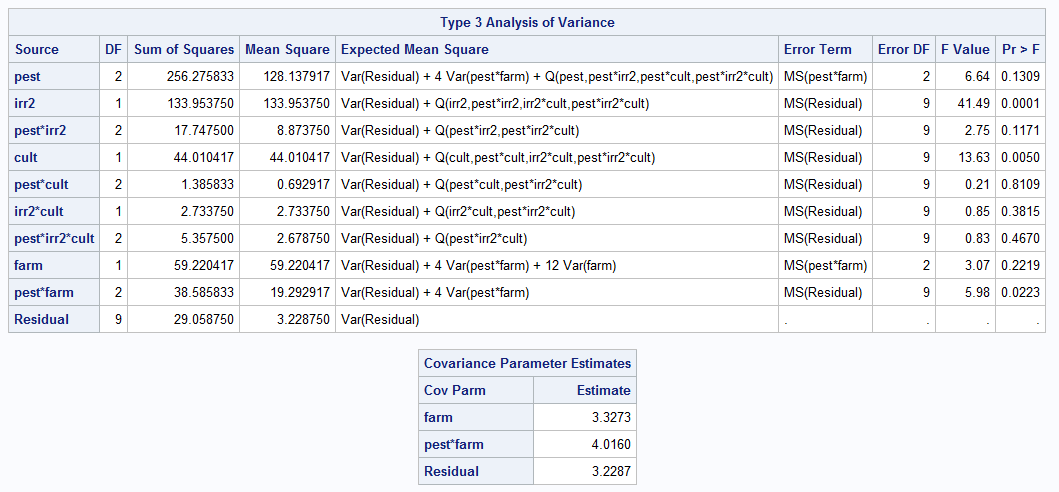
\includegraphics[scale=0.6]{CornSP6}
\end{center}


~\\
Note:  In practice, you should probably use the default method of estimation in proc mixed called REML for most mixed models.